\documentclass[unicode,11pt,a4paper,oneside,numbers=endperiod,openany]{scrartcl}
\usepackage{listings}

\renewcommand{\thesubsection}{\arabic{subsection}}

\usepackage{ifthen}
\usepackage[utf8]{inputenc}
\usepackage{graphics}
\usepackage{graphicx}
\usepackage{hyperref}

\pagestyle{plain}
\voffset -5mm
\oddsidemargin  0mm
\evensidemargin -11mm
\marginparwidth 2cm
\marginparsep 0pt
\topmargin 0mm
\headheight 0pt
\headsep 0pt
\topskip 0pt        
\textheight 255mm
\textwidth 165mm

\newcommand{\duedate} {}
\newcommand{\setduedate}[1]{%
\renewcommand\duedate {\textbf{Due date:}~ #1}}
\newcommand\isassignment {false}
\newcommand{\setassignment}{\renewcommand\isassignment {true}}
\newcommand{\ifassignment}[1]{\ifthenelse{\boolean{\isassignment}}{#1}{}}
\newcommand{\ifnotassignment}[1]{\ifthenelse{\boolean{\isassignment}}{}{#1}}

\newcommand{\assignmentpolicy}{
\begin{table}[h]
\begin{center}
\scalebox{0.8} {%
\begin{tabular}{|p{0.02cm}p{16cm}|}
\hline
&\\
\multicolumn{2}{|c|}{\Large\textbf{Numerical Computing 2023 ---  Submission Instructions}}\\
\multicolumn{2}{|c|}{\large\textbf{(Please, notice that following instructions are mandatory: }}\\
\multicolumn{2}{|c|}{\large\textbf{submissions that don't comply with, won't be considered)}}\\
&\\
\textbullet & Assignments must be submitted to \href{https://www.icorsi.ch/course/view.php?id=14666}{iCorsi} (i.e. in electronic format).\\
\textbullet & Provide both executable package and sources (e.g. C/C++ files, MATLAB). 
If you are using libraries, please add them in the file. Sources must be organized in directories called:\\
\multicolumn{2}{|c|}{\textit{Project\_number\_lastname\_firstname}}\\
& and  the  file must be called:\\
\multicolumn{2}{|c|}{\textit{project\_number\_lastname\_firstname.zip}}\\
\multicolumn{2}{|c|}{\textit{project\_number\_lastname\_firstname.pdf}}\\
\textbullet &  The TAs will grade your project by reviewing your project write-up, and looking at the implementation you attempted, and benchmarking your code's performance.\\

\textbullet & You are allowed to discuss all questions with anyone you like; however: (i) your submission must list anyone you discussed problems with and (ii) you must write up your submission independently.\\
\hline
\end{tabular}
}
\end{center}
\end{table}
}
\newcommand{\punkte}[1]{\hspace{1ex}\emph{\mdseries\hfill(#1~\ifcase#1{Points}\or{Points}\else{Points}\fi)}}


\newcommand\serieheader[6]{
\thispagestyle{empty}%
\begin{flushleft}

\includegraphics[width=0.45\textwidth]{CI_logo}
\end{flushleft}
  \noindent%
  {\large\ignorespaces{\textbf{#1}}\hspace{\fill}\ignorespaces{ \textbf{#2}}}\\ \\%
  {\large\ignorespaces #3 \hspace{\fill}\ignorespaces #4}\\
  \noindent%
  \bigskip
  \hrule\par\bigskip\noindent%
  \bigskip {\ignorespaces {\Large{\textbf{#5}}}
  \hspace{\fill}\ignorespaces \large \ifthenelse{\boolean{\isassignment}}{\duedate}{#6}}
  \hrule\par\bigskip\noindent%  \linebreak
 }

\makeatletter
\def\enumerateMod{\ifnum \@enumdepth >3 \@toodeep\else
      \advance\@enumdepth \@ne
      \edef\@enumctr{enum\romannumeral\the\@enumdepth}\list
      {\csname label\@enumctr\endcsname}{\usecounter
        {\@enumctr}%%%? the following differs from "enumerate"
	\topsep0pt%
	\partopsep0pt%
	\itemsep0pt%
	\def\makelabel##1{\hss\llap{##1}}}\fi}
\let\endenumerateMod =\endlist
\makeatother




\usepackage{textcomp}





\begin{document}


\setassignment
\setduedate{Wednesday, 8 November 2023, 11:59 PM}

\serieheader{Numerical Computing}{2023}{\textbf{Student:} Hun Rim}{\textbf{Discussed with:} Georgy Batyrev}{Solution for Project 3}{}
\newline

\assignmentpolicy


\newpage

\subsection{Spectral clustering of non-convex sets [50 points]}
\begin{enumerate} 
\item Run the Matlab function \textit{datasets/getPoints()}. A graphical output of 6 different non-convex sets will
be produced. Use this function to output the coordinate list of the different cloudpoints and replace the variable
\textit{Pts dummy} with the set you wish to cluster. Consider the set named half-kernel: can you identify the two
obvious clusters in this dataset? Describe them briefly and explain what difficulties a clustering algorithm could
eventually encounter in a scenario of this kind.\\

 \begin{figure}[h!]
    \begin{minipage}[c]{1\linewidth}
        \centering
        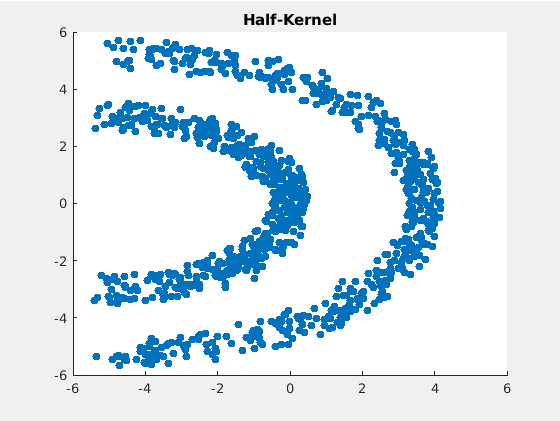
\includegraphics[width=0.8\linewidth]{./figures/halfkernel.png}
    \end{minipage}
  \caption{Graphical Output Of Half Kernel Dataset}
\end{figure}
As you can see from the graphical representation, the two clusters are very easy to spot. The first cluster is the smaller waxing crescent moon shaped collection of data points, and the second cluster is also waxing crescent moon shaped collection of data points but bigger than the first cluster and it surrounds the first cluster.\\

One example of the challenge this kind of clustering algorithm could face is incorrect partitioning of the datapoints into multiple clusters due to varying density if the algorithm relies on the density to partition. Even with the bare-eye it is clear that some parts of the graph is more densely populated than the others so it is a very possible issue. \\

Another problem can be when the cluster regions are close to each other. If the cluster regions are close, it would be very hard to differentiate separate clusters as there isn't any other factor to classify them.\\

Finally, non-convex clusters could be problematic for a basic clustering algorithm like \textbf{k-means}, as the distances between centroids are a important factor in calculating it but it is not so clear in non-convex sets. As a result, it might create an inccurate splits due to the center of the cluster which is very clustered.\\

 \item {Use the function \textit{minSpanTree()} to find the minimal spanning tree of the full graph. Use this information
to determine the ${\epsilon}$ factor for the ${\epsilon}$-similarity graph.}

Minimum span tree(MST) is the minmum subset of the edges that can connect all the vertices in an undirected graph G with \textit{n} vertices and \textit{m} edges. Spectral clustering uses eigenvalues of the similarity matrix formed from the data points to reduce number of edges, and it is very useful when identifying clusters. Unlike k-means clustering, spectral clustering is very good with identifying clusters which are not linearly separable. \\

We can define the MST and find the ${\epsilon}$ as following:\\
 \begin{lstlisting}[language=Matlab]
    G = pdist2(Pts_halfk, Pts_halfk);
    A = double(G < max(G(:)));
    MST = minSpanTree(A);
    eps = max(MST(MST > 0));
 \end{lstlisting}
 
 The following is the plotted graph of MST.
 
 
  \begin{figure}[h!]
    \begin{minipage}[c]{1\linewidth}
        \centering
        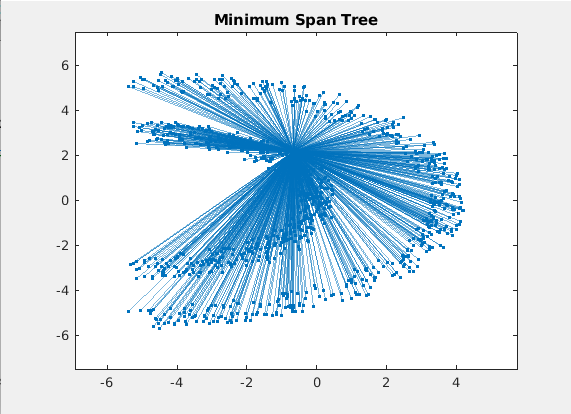
\includegraphics[width=0.8\linewidth]{./figures/minSpanTree.png}
    \end{minipage}
  \caption{Plotted Minimum Span Tree of Half Kernel}
\end{figure}

 \item Complete the Matlab function \textit{epsilonSimGraph()}. It should generate the similarity matrix of the ${\epsilon}$-similarity graph. \\
 
\begin{lstlisting}[language=Matlab]
    n = size(Pts, 1);
    G = zeros(n, n);

    for i = 1:n
        for j = 1:n
            if i == j
                continue;
            end

            distance = norm(Pts(i, :) - Pts(j, :));

            if distance < epsilon
                G(i, j) = 1;
            end
        end

    end
\end{lstlisting}

The \textit{epsilonSimGraph()} can be completed like above to generate the similarity matrix of the ${\epsilon}$-similarity graph.

The epsilon similarity graph is constructed by only connecting points which has distance less than epsilson units to emphasize the local neighborhood structure. \\

\vspace{20px}

\item {Create the adjacency matrix for the ${\epsilon}$ similarity graph and visualize the resulting graph using the function
\textit{gplotg()}.} \\

Like the name states, adjacency matrix denotes the neighbor relation between the nodes and states which vertices are next(adjacent) to other vertices. Because in an unweighted graph, the presence of adjacency is represented with binary, we can do the following to get an adjacency graph: \\


\begin{lstlisting}[language=Matlab]
    W = double(D < eps);
\end{lstlisting}
\vspace{20px}
According to the implementation, the adjacency graph looks like the following. \\

  \begin{figure}[h!]
    \begin{minipage}[c]{1\linewidth}
        \centering
        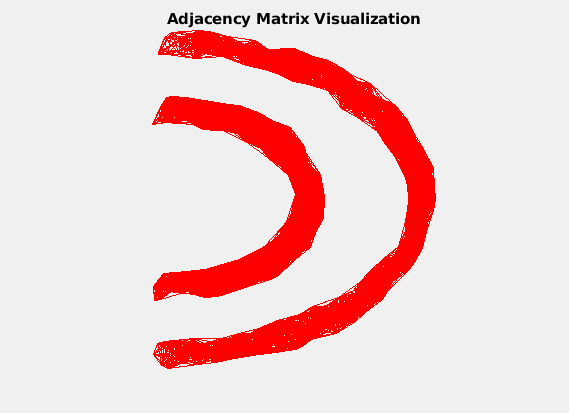
\includegraphics[width=0.8\linewidth]{./figures/adjacency.png}
    \end{minipage}
  \caption{Adjacency Matrix Visualization}
\end{figure}

\item{Create the Laplacian matrix and implement spectral clustering. Your goal is to find the eigenvectors of the
Laplacian corresponding to the ${K = 2}$ smallest eigenvalues. Afterwards, use the function ${kmeans\_mod()}$ to
cluster the rows of these eigenvectors.} \\

The implementation is as following:\\

\begin{lstlisting}[language=Matlab]
    [L,Diag] = CreateLapl(W);
    [eigVec, eigVal] = eig(L);
    [sortedEigVal, ind] = sort(diag(eigVal));
    H = eigVec(:, ind(1:K));
    H_normalized = diag(1./sqrt(sum(H.^2, 2))) * H;
\end{lstlisting}

Then we just have to replace dummy value with ${H\_normalized}$ we obtained.

\item{Use the ${kmeans\_mod()}$ function to perform k-means clustering on the input points. Visualize the two clustering results using the function \textit{gplotmap()}. You can debug your implementation by using as a reference the
results reported in Figure 1, which are relative to the half-kernel dataset.} \\

  \begin{figure}[h!]
    \begin{minipage}[c]{1\linewidth}
        \centering
        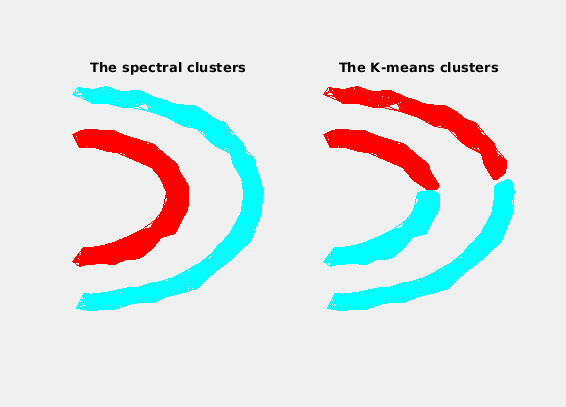
\includegraphics[width=0.8\linewidth]{./figures/half_k_clusters.png}
    \end{minipage}
  \caption{Half-kernel dataset in spectral clusters(left) and K-means-clusters(right), ${K=2}$}
\end{figure}

\vspace{20px}

\item {Cluster the datasets ${i)}$ Two spirals, ${ii)}$ Cluster in cluster, and ${iii)}$ Crescent ${\&}$ full moon in ${K=2}$ clusters, and
visualize the results obtained with spectral clustering and k-means directly on the input data. Do the same for
${i)}$ Corners, and ${ii)}$ Outlier for ${K=4)}$ clusters.}\\

\textit{To get the results, I am manually manipulating the values of the script.}

\newpage
1) ${K=2}$
  \begin{figure}[h!]
    \begin{minipage}[c]{1\linewidth}
        \centering
        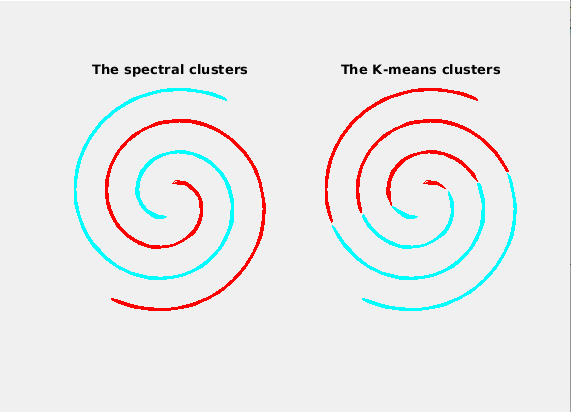
\includegraphics[width=0.6\linewidth]{./figures/twospiralcluster.png}
    \end{minipage}
  \caption{Two Spirals dataset in spectral clusters(left) and K-means-clusters(right), ${K=2}$}
\end{figure}

\begin{figure}[h!]
    \begin{minipage}[c]{1\linewidth}
        \centering
        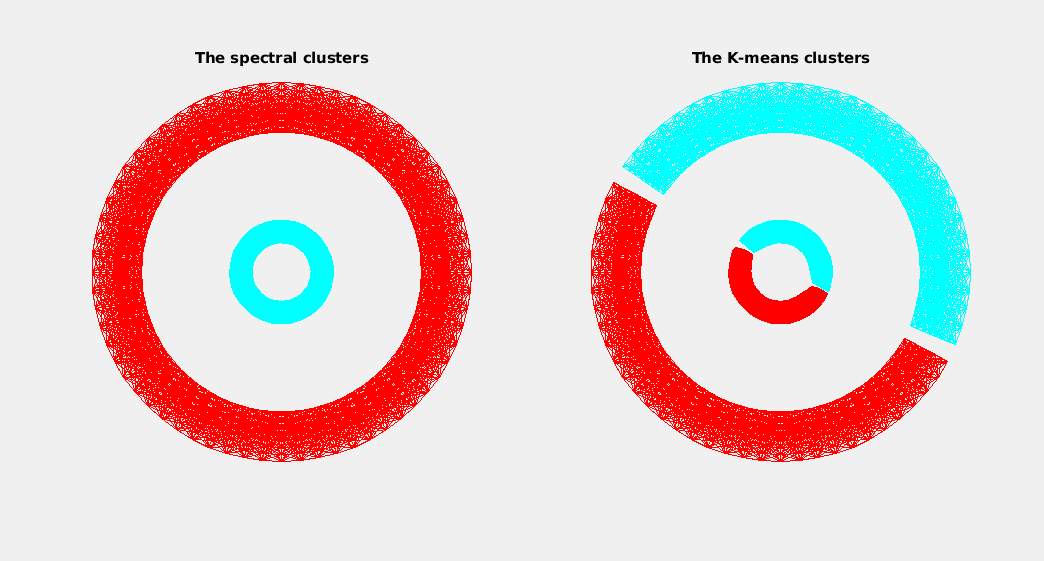
\includegraphics[width=0.6\linewidth]{./figures/clusterincluster.png}
    \end{minipage}
  \caption{Cluster in cluster dataset in spectral clusters(left) and K-means-clusters(right), ${K=2}$}
\end{figure}

\begin{figure}[h!]
    \begin{minipage}[c]{1\linewidth}
        \centering
        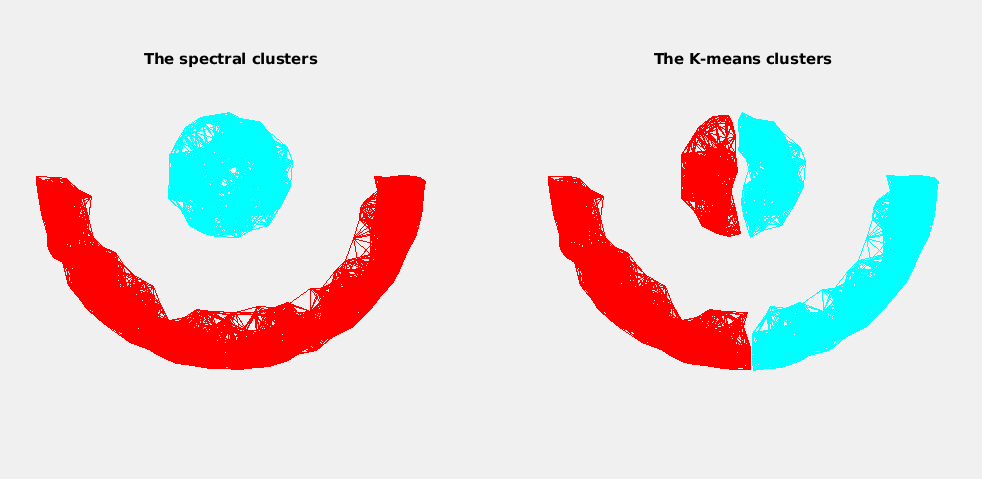
\includegraphics[width=0.6\linewidth]{./figures/fullmoon.png}
    \end{minipage}
  \caption{Crescent full moon dataset in spectral clusters(left) and K-means-clusters(right), ${K=2}$}
\end{figure}

\newpage

2) ${K=4}$
\begin{figure}[h!]
    \begin{minipage}[c]{1\linewidth}
        \centering
        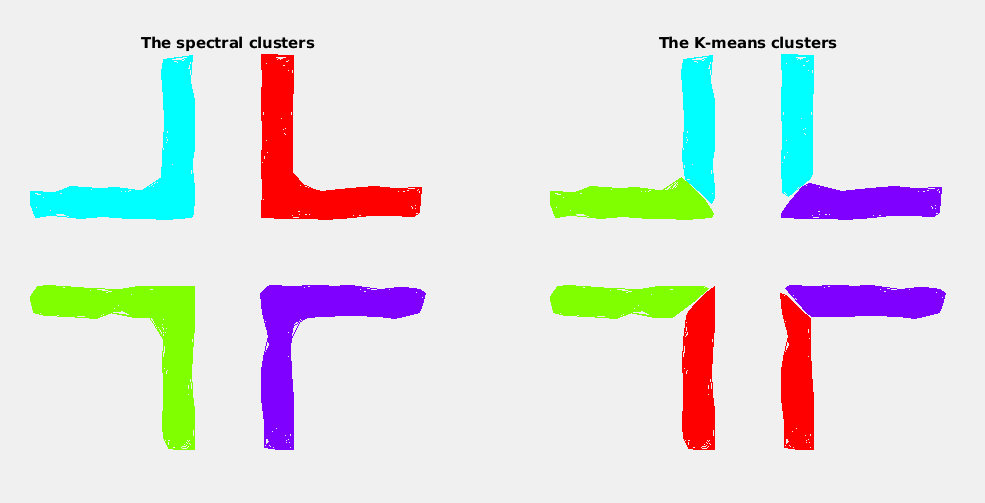
\includegraphics[width=0.6\linewidth]{./figures/corners4.png}
    \end{minipage}
  \caption{Cluster in cluster dataset in spectral clusters(left) and K-means-clusters(right), ${K=2}$}
\end{figure}

\begin{figure}[h!]
    \begin{minipage}[c]{1\linewidth}
        \centering
        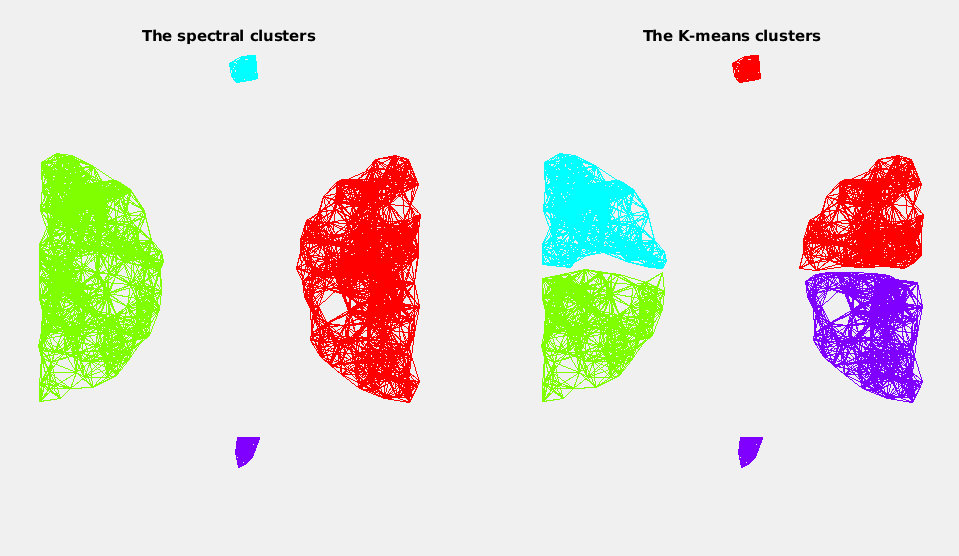
\includegraphics[width=0.6\linewidth]{./figures/outlier4.png}
    \end{minipage}
  \caption{Cluster in cluster dataset in spectral clusters(left) and K-means-clusters(right), ${K=2}$}
\end{figure}

\end{enumerate}


 \newpage
\subsection{Spectral clustering of real-world graphs [35 points]}
\begin{enumerate}
 \item Construct the Laplacian matrix, and draw the graphs using the eigenvectors to supply coordinates. Locate vertex
${i}$ at position: \\

 \begin{center}
  \begin{math}
 (x_i, y_i) = (v_2(i), v_3(i))
\end{math}
 \end{center}

where ${v2, v3}$ are the eigenvectors associated with the 2nd and 3rd smallest eigenvalues. Figure 2 illustrates
these 2 ways of visualizing the \textit{airfoil1} graph. Plot your results for all the three additionally supplied meshes,
grid2, barth, 3elt. \\

1) \textit{grid2}
\begin{figure}[h!]
    \begin{minipage}[c]{1\linewidth}
        \centering
        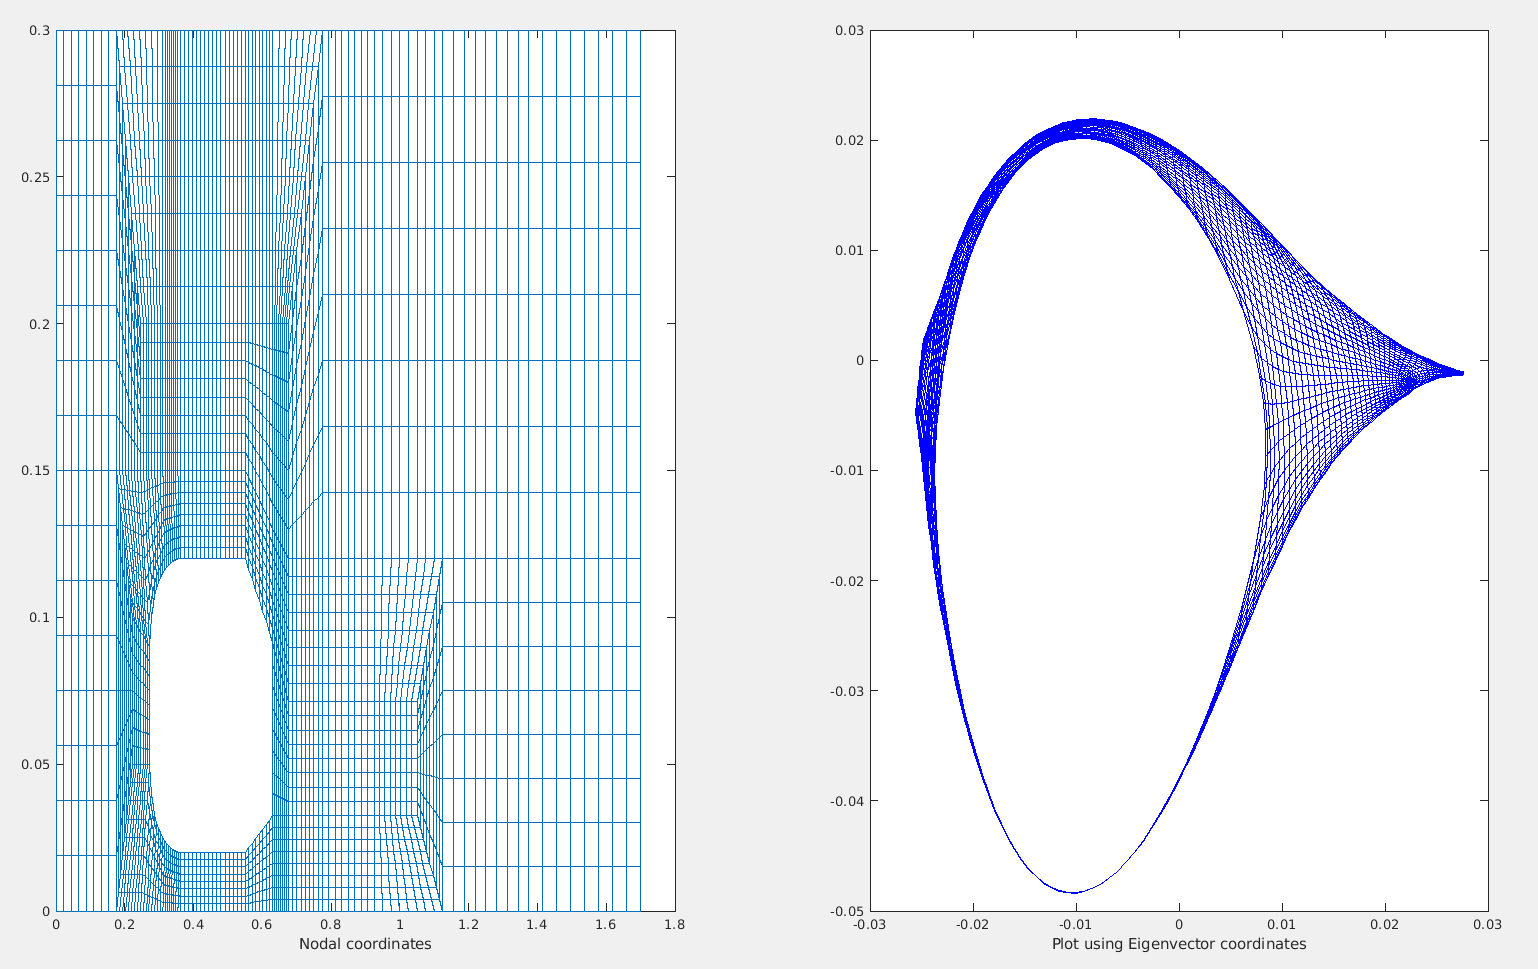
\includegraphics[width=0.6\linewidth]{./figures/grid2.png}
    \end{minipage}
  \caption{Nodal coordinates(left), Eigenvectors(right)}
\end{figure}


2) \textit{barth}
\begin{figure}[h!]
    \begin{minipage}[c]{1\linewidth}
        \centering
        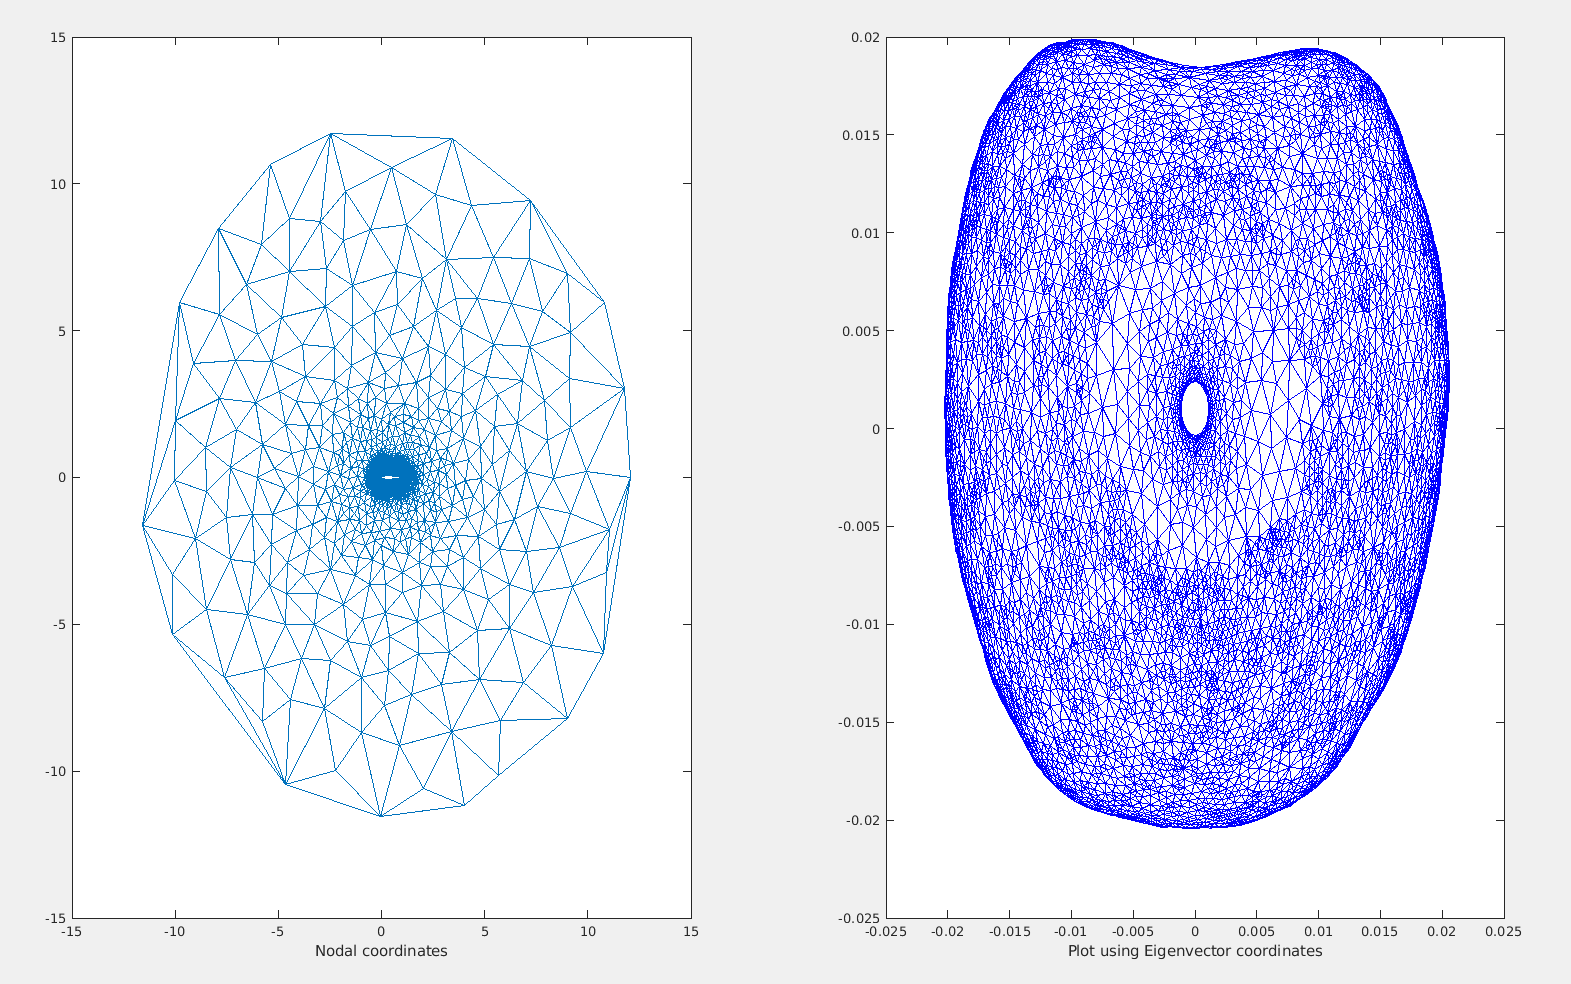
\includegraphics[width=0.6\linewidth]{./figures/barth.png}
    \end{minipage}
  \caption{Nodal coordinates(left), Eigenvectors(right)}
\end{figure}

\newpage
3) \textit{3elt}
\begin{figure}[h!]
    \begin{minipage}[c]{1\linewidth}
        \centering
        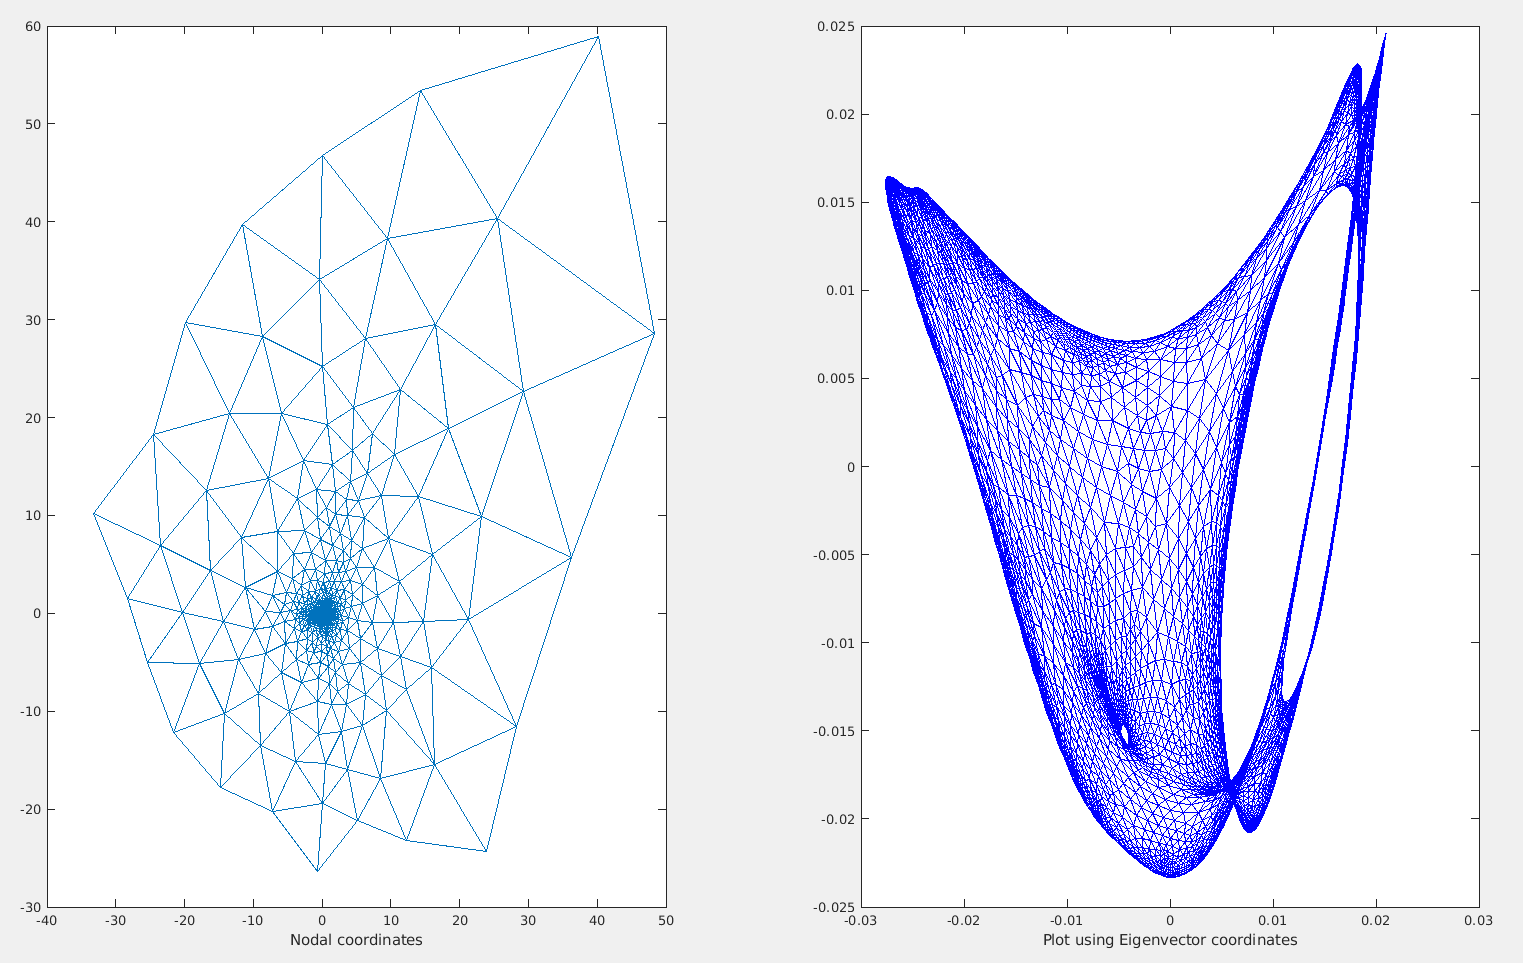
\includegraphics[width=0.6\linewidth]{./figures/3elt.png}
    \end{minipage}
  \caption{Nodal coordinates(left), Eigenvectors(right)}
\end{figure}

\vspace{50px}
\item {Cluster each graph in K = 4 clusters with the spectral and the k-means method. Plot all of your results and
describe the differences that you can see in the output of the 2 different algorithms and where they might come
from. } \\

\vspace{20px}

1) \textit{grid2}
\begin{figure}[h!]
    \begin{minipage}[c]{1\linewidth}
        \centering
        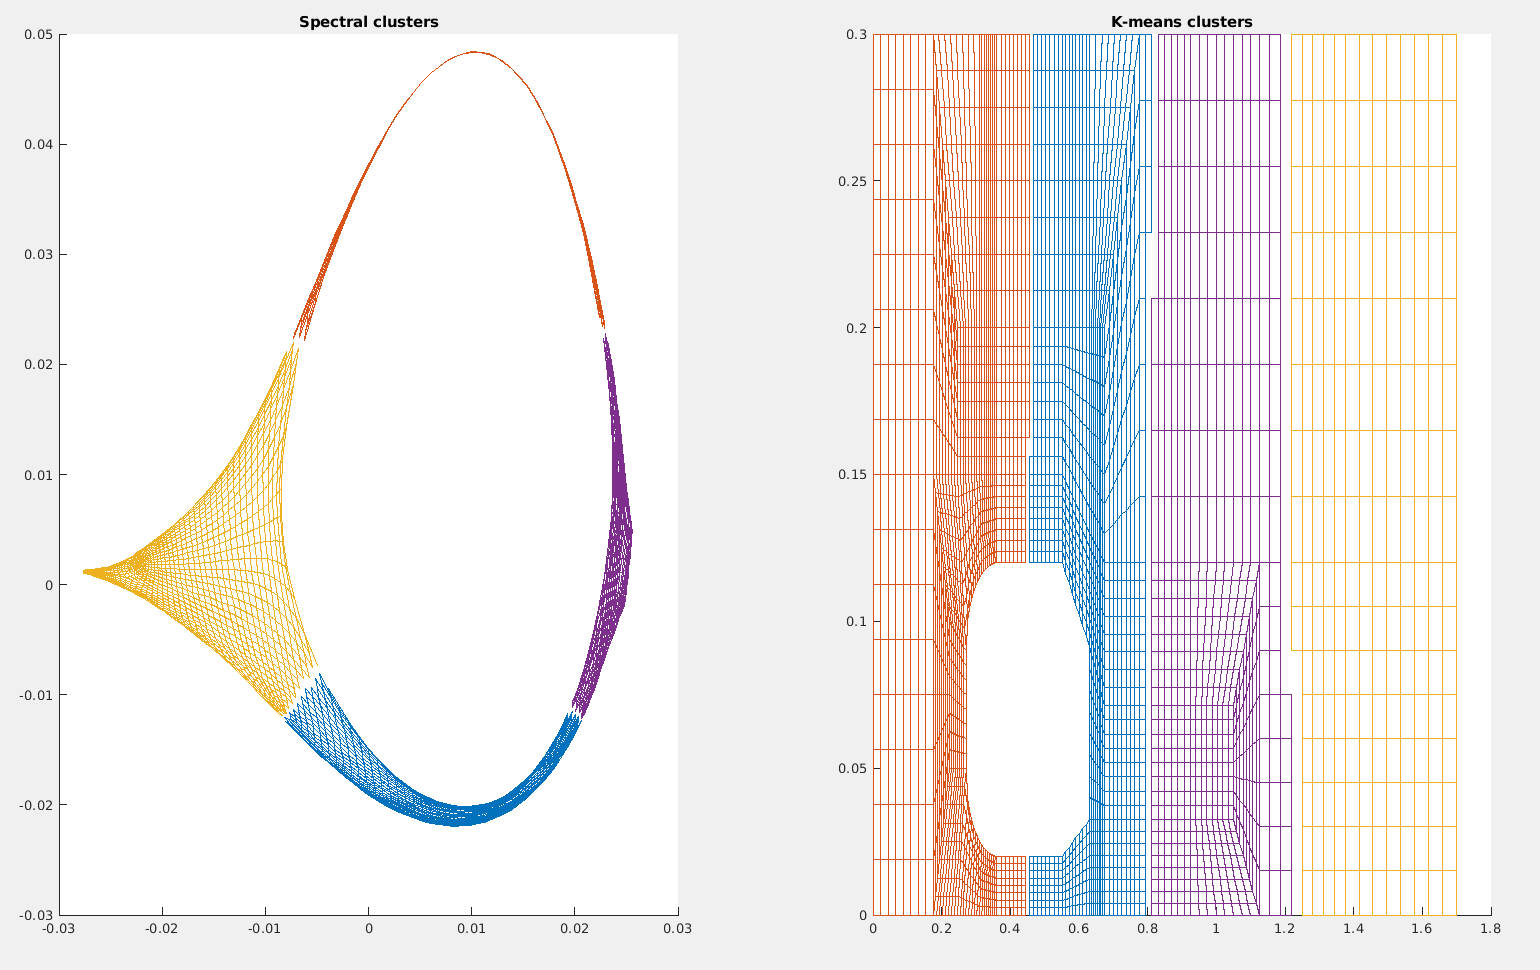
\includegraphics[width=0.6\linewidth]{./figures/grid2Cluster.png}
    \end{minipage}
  \caption{Spectral Clusters(left), K-mean Clusters(right)}
\end{figure}

\newpage
2) \textit{barth}
\begin{figure}[h!]
    \begin{minipage}[c]{1\linewidth}
        \centering
        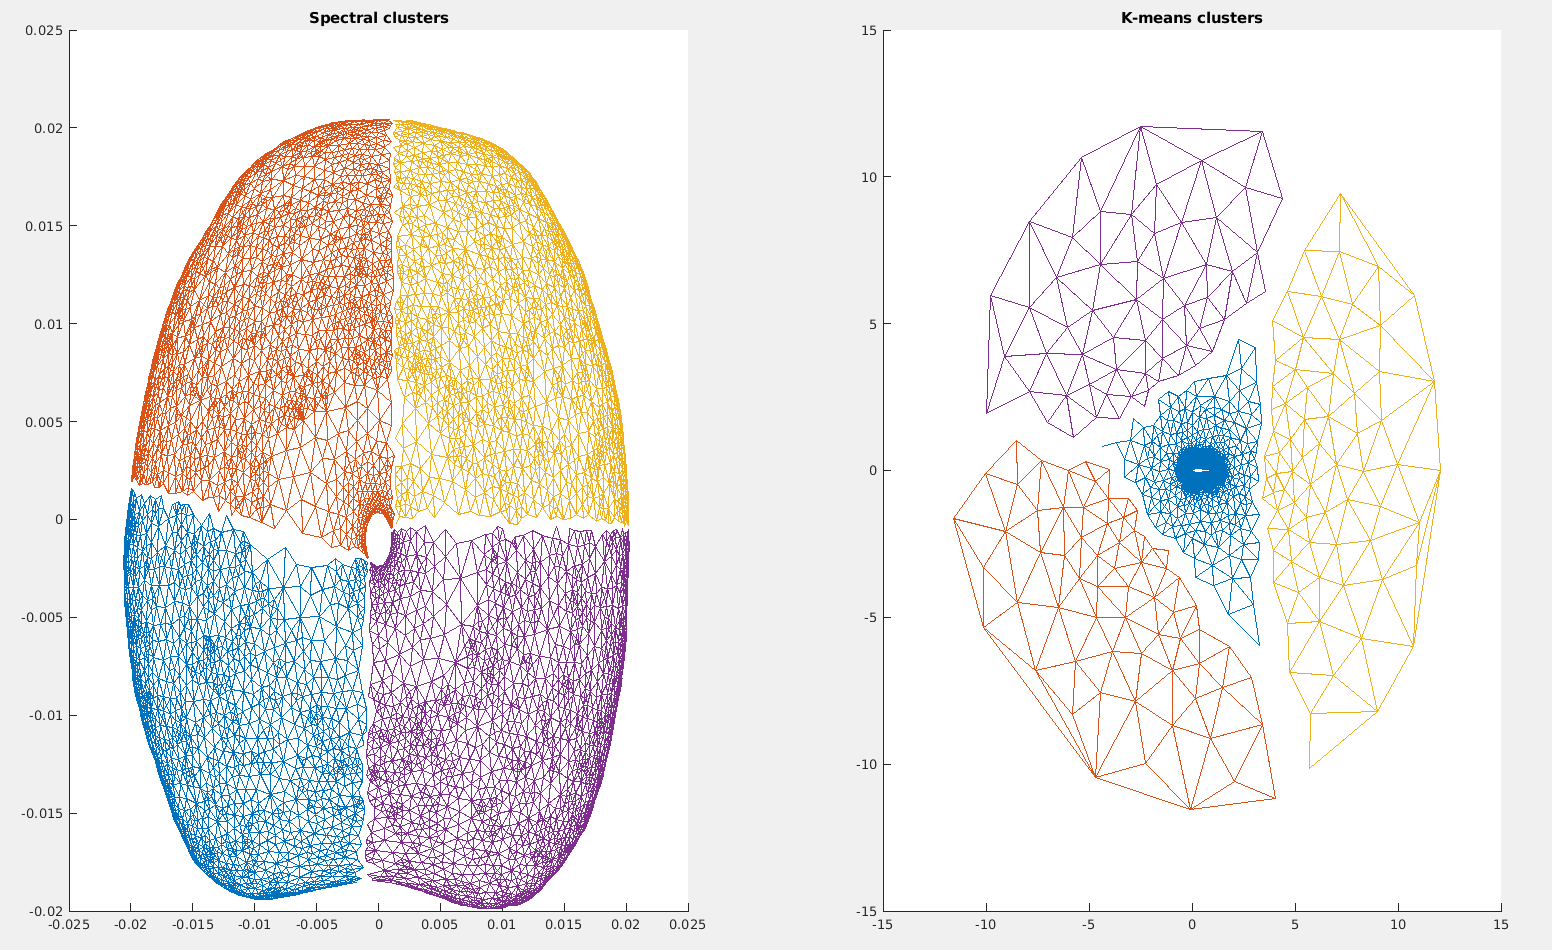
\includegraphics[width=0.6\linewidth]{./figures/barthCluster.png}
    \end{minipage}
  \caption{Spectral Clusters(left), K-mean Clusters(right)}
\end{figure}

3) \textit{3elt}
\begin{figure}[h!]
    \begin{minipage}[c]{1\linewidth}
        \centering
        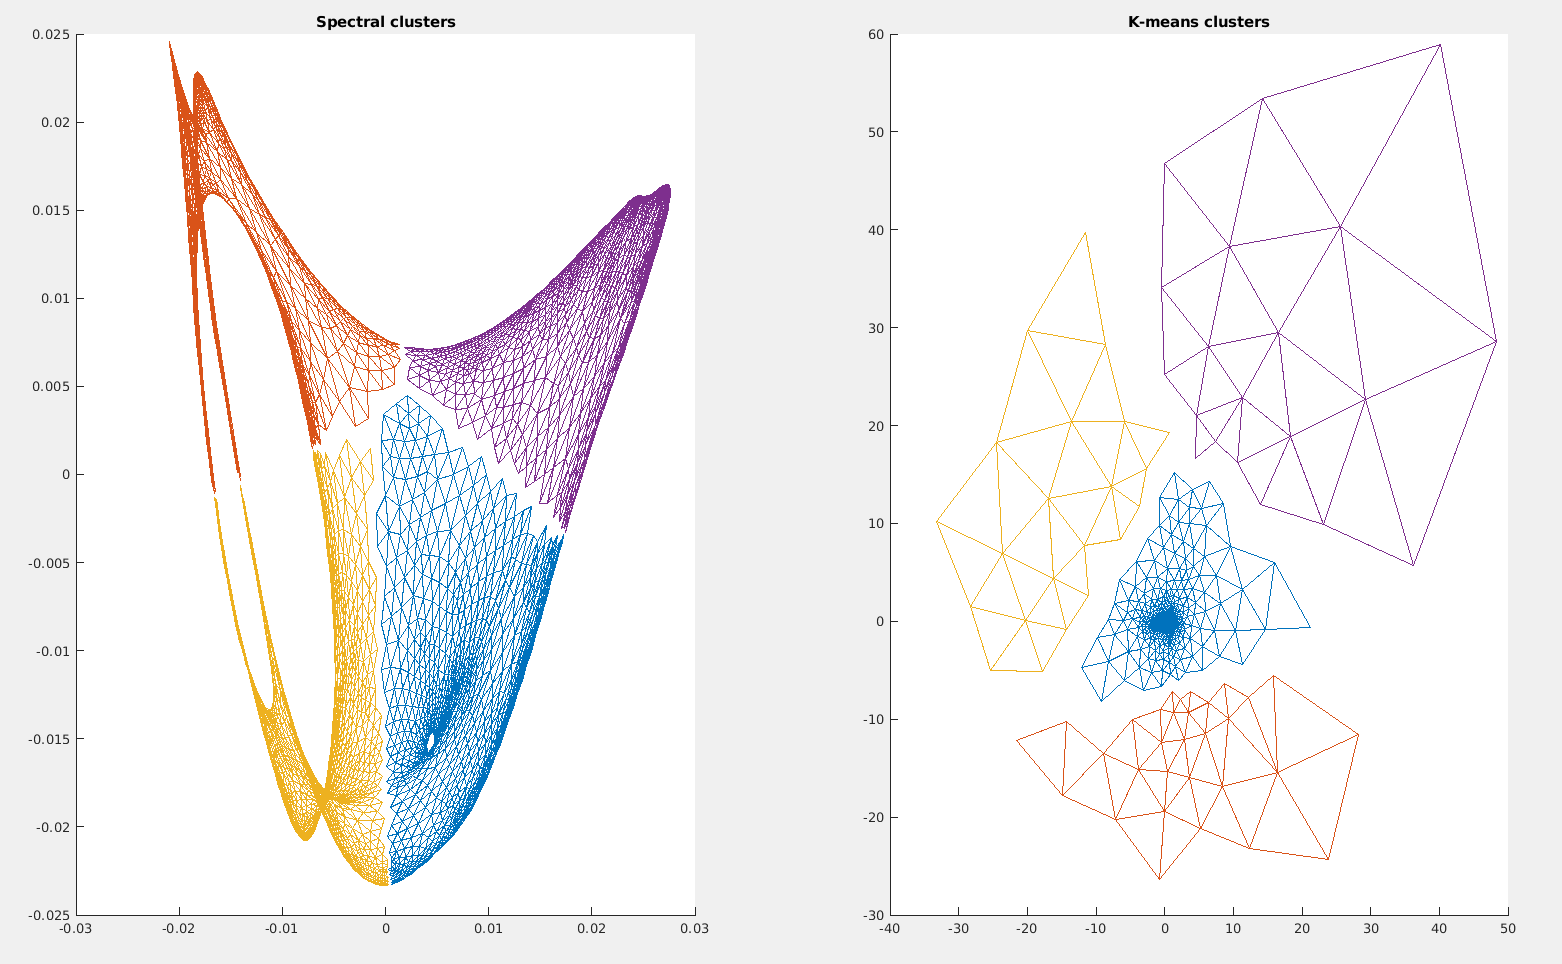
\includegraphics[width=0.6\linewidth]{./figures/3eltCluster.png}
    \end{minipage}
  \caption{Spectral Clusters(left), K-mean Clusters(right)}
\end{figure}

Even though K-means is also able to create clusters, the clusters are unbalanced with some high density areas and some significantly lower density areas. (Density, as in number of nodes in a given area) \\

On the otherhand, spectral clusters have a balanced graph with similar density level all over the graph. K-means clusters are unbalanced because it is not as smart as the spectral. K-means is incapable of recognizing densities and just creates clusters within a defined radius, hence, creating an unbalanced clusters. \\

\item {Report in the table below, the number of nodes per cluster and plot a histogram. What can you observe?} \\


\begin{figure}
\begin{center}
\begin{tabular}{|l|r|r|} \hline
Case & Spectral & K-means \\
\hline
grid2 & 1361 & 604 \\
\hline
barth & 1861 & 59 \\
\hline
3elt & 1814 & 3010 \\
\hline
 
\end{tabular}
\end{center}
\caption{Number of nodes per cluster when ${K=4}$}
\end{figure}


\begin{figure}[h!]
    \begin{minipage}[c]{1\linewidth}
        \centering
        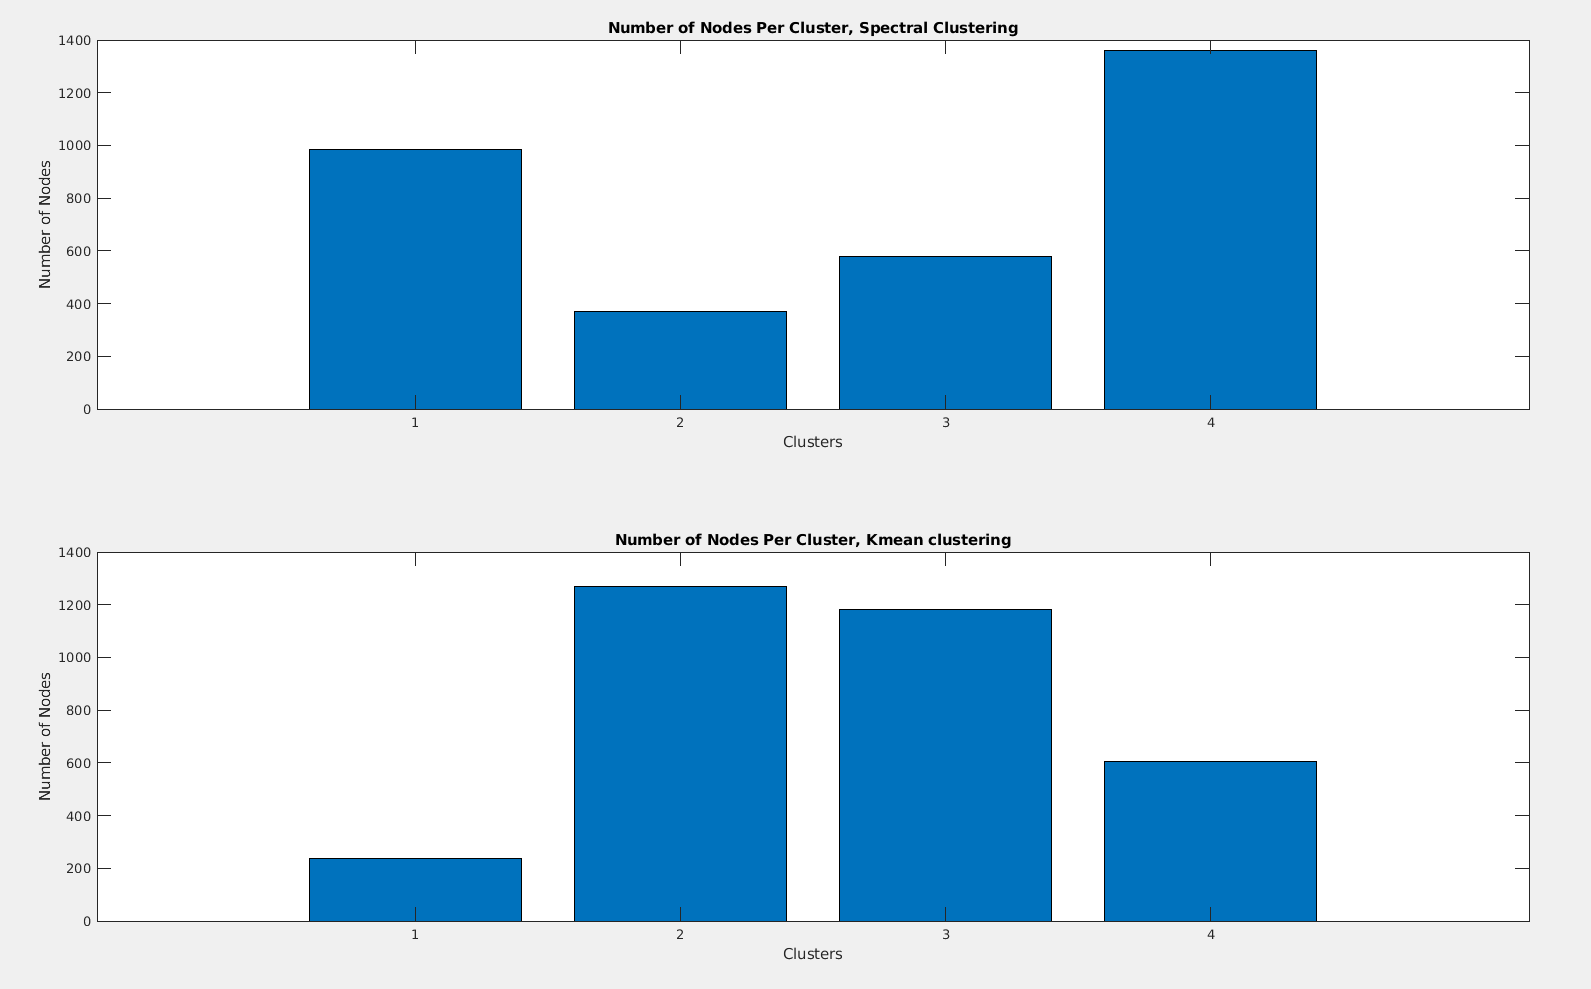
\includegraphics[width=0.4\linewidth]{./figures/grid2Histogram.png}
    \end{minipage}
  \caption{Spectral Clusters Histogram(top), K-mean Clusters Histogram(bottom), grid2 dataset}
\end{figure}

\begin{figure}[h!]
    \begin{minipage}[c]{1\linewidth}
        \centering
        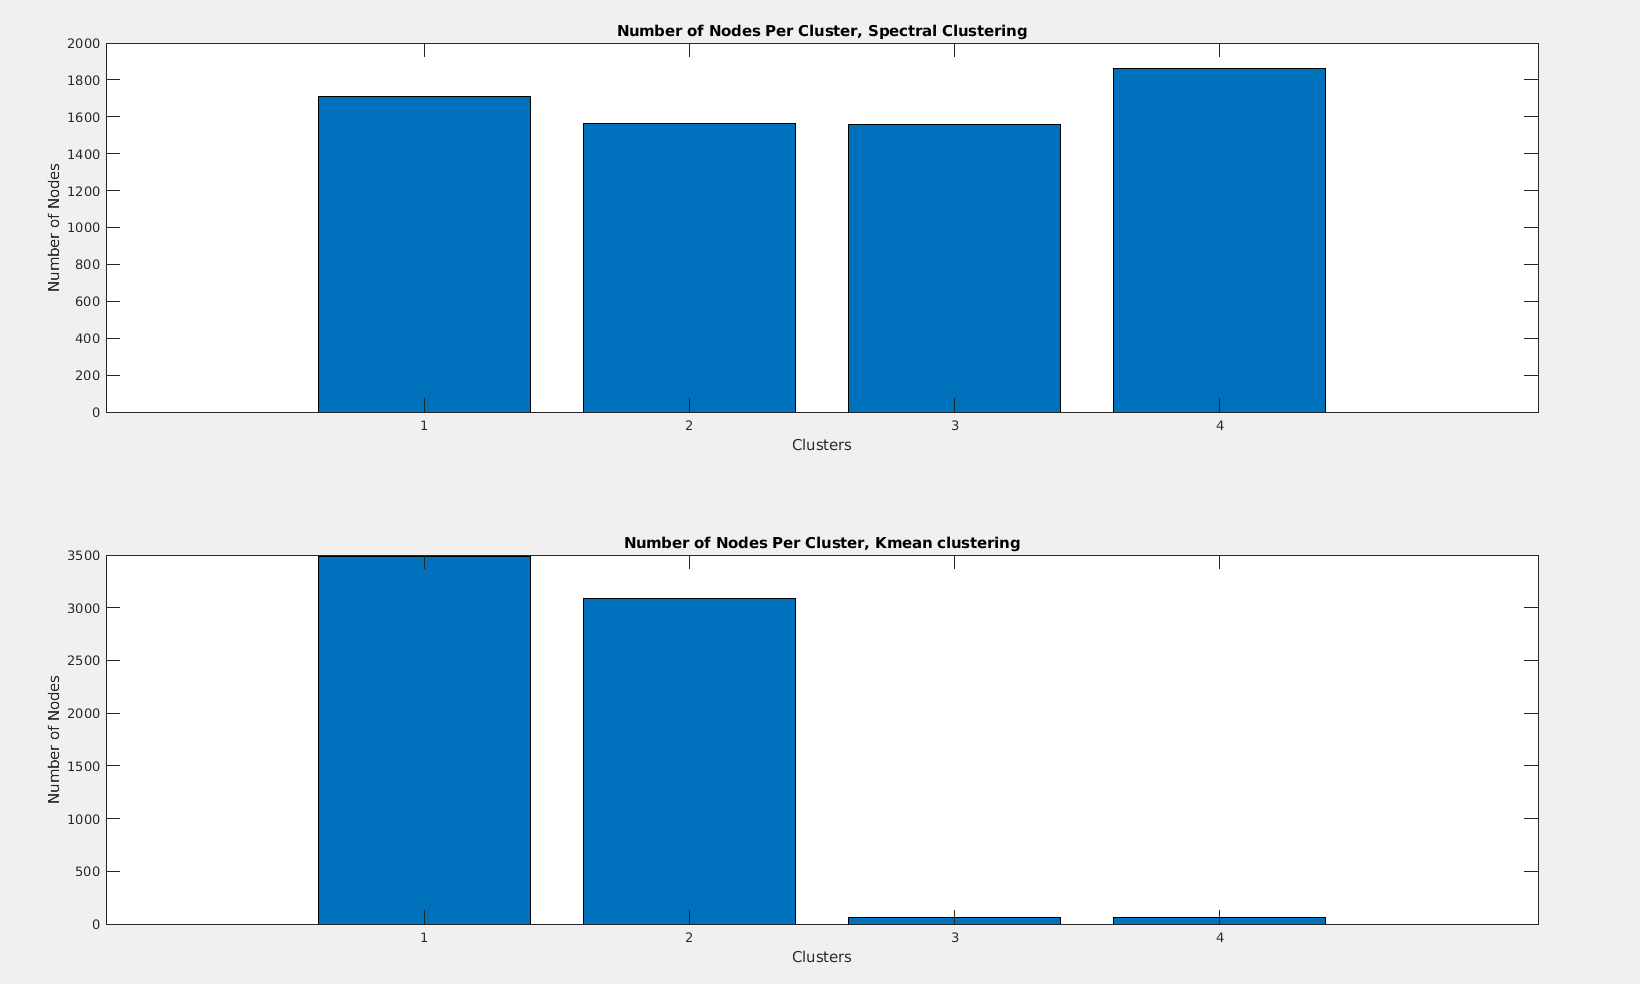
\includegraphics[width=0.4\linewidth]{./figures/barthHistogram.png}
    \end{minipage}
  \caption{Spectral Clusters Histogram(top), K-mean Clusters Histogram(bottom), Barth dataset}
\end{figure}

\begin{figure}[h!]
    \begin{minipage}[c]{1\linewidth}
        \centering
        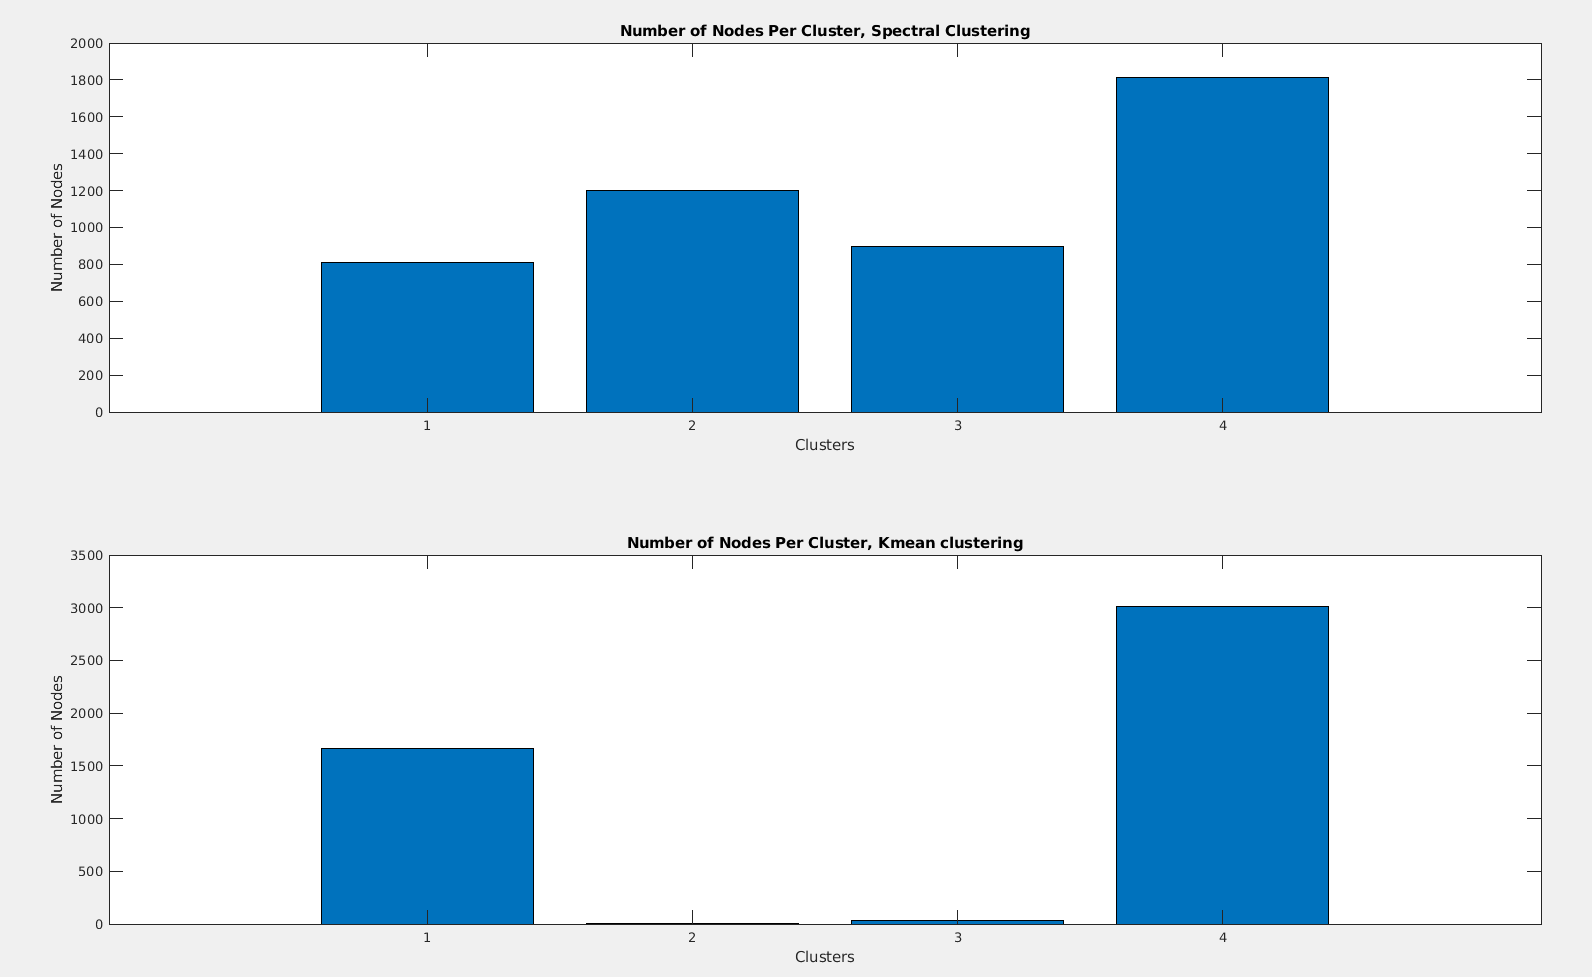
\includegraphics[width=0.4\linewidth]{./figures/3eltHistogram.png}
    \end{minipage}
  \caption{Spectral Clusters Histogram(top), K-mean Clusters Histogram(bottom), 3elt dataset}
\end{figure}

{From the observation of the histograms, in general, the spread nodes per cluster in spectral clustering is more balanced than the spread of nodes per cluster in K-mean clustering. Which matches the observation made in the previous question from the cluster graphs.}


\end{enumerate}




\end{document}
